\documentclass{scrartcl}
\usepackage[top=3cm, bottom=3cm, left=2cm,right=2cm]{geometry} 

\usepackage[english]{babel}
\usepackage[utf8]{inputenc}
\usepackage{mathtools}
\usepackage{esvect}
\usepackage{amssymb}
\usepackage{amsmath}

\usepackage{dcolumn}
\usepackage{booktabs}
\usepackage{tikz}
\usepackage{graphicx}
\usepackage{multicol}
\usepackage{float}
\usepackage{url}

\usepackage{listings}

%multiline comments
\usepackage{verbatim}

\usetikzlibrary{positioning,shapes,arrows}

\DeclareMathOperator*{\argmin}{argmin} % no space, limits underneath in displays
\DeclareMathOperator*{\argmax}{argmax} % no space, limits underneath in displays

\DeclarePairedDelimiter\abs{\lvert}{\rvert}%
\DeclarePairedDelimiter\norm{\lVert}{\rVert}%

\usepackage{titlesec}
\newcommand{\sectionbreak}{\clearpage}

\usepackage[parfill]{parskip}
\parskip = 4pt

\title{Künstliche Intelligenz 2 - Summary}
\author{Sebastian Rietsch}

\begin{document}
\maketitle

\section{Probablistic Reasoning, Part I: Basics}
\subsection{Introduction}
\textbf{Sources of Uncertainty} in Decision-Making:
\begin{itemize}
    \item
        Non-deterministic actions
    \item
        Partial observability with unreliable sensors
    \item
        Uncertainty about the domain behavior
\end{itemize}

What is \textbf{probabilistic reasoning}?
\begin{itemize}
    \item
        Deducing probabilities from knowledge about \textit{other} probabilities
    \item
        Determines probabilities that are difficult to assess, based on probabilities that are (relatively) easy to assess (\textit{to asses:} the process of estimating a probability \(P\) using statistics)
\end{itemize}

\textbf{Rational Agents}:
\begin{itemize}
    \item
        We have a choice of \textbf{actions}
    \item
        These can lead to different solutions with different probabilities
    \item
        The actions have different costs
    \item
        The results have different utilities
    \item
        A rational agent chooses the action with the \textbf{maximum expected utility}
\end{itemize}

\subsection{Unconditional Probabilities}
A \textbf{probability theory} is an assertion language for talking about possible worlds and an inference method for quantifying the degree of belief in such assertions (Example: we roll two dice with six sides, then we have 36 possible worlds: \((1,1), (2,1), \dots, (6,6)\)).

A \textbf{probability model} \(\langle \Omega, P \rangle\) consists of a set \(\Omega\) of possible worlds called the sample space and a probability function \(P: \Omega \rightarrow \mathbb{R}\), such that \(0 \leq P(\omega) \leq 1\) for all \(\omega \in \Omega\) and \(\sum_{\omega \in \Omega} P(\omega) = 1\). We restrict ourselves to a discrete, countable sample space.

\textbf{Random variables}:
\begin{itemize}
    \item
        A random variable is a variable quantity whose value depends on possible outcomes of unknown variables and processes we do not understand
    \item
        Given a random variable \(X\), \(P(X = x)\) denotes the prior probability, or unconditional probability, that \(X\) has value \(x\)
    \item
        We will refer to the fact \(X = x\) as an event or outcome
    \item
        For Boolean variable \(Name\), we write name for \(Name = \top\) and \(\lnot name\) for \(Name = \bot\)
\end{itemize}

The \textbf{probability distribution} for a random variable \(X\), written \(P(X)\), is the vector of probabilities for the (ordered) domain of \(X\).

Given a subset \(Z \subseteq \{X_1, \dots, X_n\}\) of random variables, an event is an assignment of values to the variables in \(Z\). The \textbf{joint probability distribution}, written \(P(Z)\), lists the probabilities of all events.

An \textbf{atomic event} is an assignment of values to all variables.

A \textbf{proposition} describes a set of multiple atomic events (\textbf{Example:} we roll two dice and are interested in the cases where they add up to 11). The probability associated with a proposition is defined by the sum of probabilities of the worlds in which it holds: For any proposition \(\phi, P(\phi) = \sum_{\omega \in \phi} P(\phi)\).

\textbf{Kolmogorov axioms:}
\begin{enumerate}
    \item
        The probability of an event is a non-negative real number: \[P(E) \in \mathbb{R}, P(E) \geq 0, \forall E \in F\] where \(F\) is the event space.
    \item
        The probability that at least one of the elementary events in the entire sample space will occure is 1: \(P(\Omega) = 1\).
    \item
        Any countable sequence of disjoint sets (mutually exclusive events) \(E_1, E_2, \dots \) satisfies \[P(\bigcup_{i=1}^{\infty} (E_i)) = \sum_{i=1}^{\infty} P(E_i).\]
\end{enumerate}
From this follows \(P(A \lor B) = P(A) + P(B) - P(A \land B)\).

\subsection{Conditional Probabilities}
In the presence of additional information, we can no loger use the unconditional (\textbf{prior}) probabilities (because probabilies model our belief, thus they depend on our knowledge).

Given propositions \(A\) and \(B\), \(P(a|b)\) denotes the \textbf{conditional probability} of \(a\) given that all we know is \(b\). The conditional, or posterior probability of \(a\) given \(b\) is defined as:
\[P(a|b) = \frac{P(a \land b)}{P(b)}\]

The \textbf{conditional probability distribution} of \(P(X|Y)\) is the table of all conditional probabilies of values of \(X\) given values of \(Y\).

\subsection{Independence}
Problem with full joint probility distributions: Given \(n\) random variables with \(k\) values each, the joint pdf containts \(k^n\) probabilities. This motivates the use of conditional probabilities while exploiting the \textbf{(conditional) independence} property.

Events \(a\) and \(b\) are \textbf{independent} if \(P(a \land b) = P(a) \cdot P(b)\), from which follows that \(P(a | b) = P(a)\) and vice versa.

In case of independence, the joint probability distribution of multiple variables can be reconstructed from smaller, statistically independent joint probability distributions.

\subsection{Basic Probabilistic Reasoning Methods}
\begin{itemize}
    \item
        \textbf{Product Rule:} \(P(a \land b) = P(a | b) P(b)\) 
    \item
        \textbf{Chain Rule:} \(P(X_1, \dots, X_n) = P(X_n | X_{n-1}, \dots X_1) \cdot \dots \cdot P(X_2 | X_1) \cdot P(X_1)\) (This works for any ordering of the variables)
    \item
        \textbf{Marginalization:} Given sets \(X\) and \(Y\) of random variables, we have:
        \[P(X) = \sum_{y \in Y} P(X, y)\]
    \item
        \textbf{Normalization:} Given a vector \(\langle w_1, \dots, w_k \rangle\) of numbers in \([0,1]\) where \(\sum_{i=1}^k w_i \leq 1\), the normalization constant \(\alpha\) is \(\alpha \langle w_1, \dots, w_k \rangle = 1/\sum_{i=1}^k w_i\)
        \begin{itemize}
            \item
                Given a random variable \(X\) and an event \(e\), we have \(P(X|e) = \alpha P(X, e)\) with \(\alpha = 1/P(e)\)
            \item
                Normalization + Marginalization: Given "query variable" \(X\), "observed event" \(e\), and "hidden variables" set \(Y\):
                \[P(X|e) = \alpha P(X, e) = \alpha \sum_{y \in Y} P(X, e, y)\]
        \end{itemize}
\end{itemize}

\subsection{Bayes' Rule}
Given propositions \(A\) and \(B\) where \(P(a) \neq 0\) and  \(P(b) \neq 0\), we have:
\[P(a|b) = \frac{P(b|a) P(a)}{P(b)}\]

\subsection{Conditional Independence}
Given sets of random variables \(Z_1, Z_2 \text{ and } Z\), we say \(Z_1\) and \(Z_2\) are \textbf{conditionally independent given \(Z\)} if:
\[P(Z_1, Z_2 | Z) = P(Z_1 | Z) \cdot P(Z_2 | Z)\]

If \(Z_1\) and \(Z_2\) are conditionally independent given \(Z\), the \(P(Z_1 | Z_2, Z) = P(Z_1 | Z)\).

\subsection{Summary}
\begin{itemize}
    \item
        Uncertainty is unavoidable in many environsments, namely whenever agents do not have perfect knowledge
    \item
        Probabilities express the degree of belief of an agent, given its knowledge, into an event
    \item
        Conditional probabilities express the likelihood of an event given observed evidence
    \item
        Assessing a probability means to use statistics to approximate the likelihood of an event
    \item
        Bayes' rule allows us to derive, from probabilities that are easy to assess, probabilities that arn't easy to assess
    \item
        Given mulitple evidence, we can exploit conditional independencie
\end{itemize}

\section{Probabilistic Reasoning, Part II: Bayesian Networks}
\subsection{What is a Bayesian Network}
Given random variables \(X_1, \dots, X_n\) with finite domains \(D_1, \dots, D_n\), a \textbf{Bayesian network} is an acyclic directed graph \(BN = \langle \{X_1, \dots, X_n\}, E\rangle\). We denote \(Parents(X_i) = \{X_j | (X_j, X_i) \in E \}\). Each \(X_i\) is associated with a function \(CPT(X_i): D_i \times \prod_{X_j \in Parents(X_i)} D_j \rightarrow [0,1]\), the \textbf{conditional probability table}. Is is a so called \textbf{graphical model}.

A node \(X\) is conditionally independent of its non-descendants (nicht Nachkommen) given its parents. A node \(X\) is conditionally independent of all other nodes in the network given its Markov blanket (parents, children, and children's parents).

\subsection{Recovering the Full Joint Probability Distribution}

\textbf{Chain rule:} For any ordering \(X_1, \dots, X_n\) we have
\[P(X_1, \dots, X_n) = P(X_n | X_{n-1} \dots, X_1) \cdot P(X_{n-1} | X_{n-2} \dots, X_1) \dots P(X_1)\]
Choose \(X_1, \dots, X_n\) consistent with \(BN: X_j \in Parents(X_i) \Rightarrow j<i\) 

With \(BN\) assumption, we can use \(P(X_i|Parents(X_i))\), instead of \(P(X_i| X_{i-1} \dots X_1)\):
\[P(X_1, \dots, X_n) = \prod_{i=1}^n P(X_i | Parents(X_i))\]

\subsection{Constructing Bayesian Networks}
Reminder: Conditional Independence 

Events \(R\) and \(B\) are conditionally independent given \(Y\) if and only if \(P(R, B | Y) = P(R|Y)P(B|Y)\) or equivalently \(P(R|B,Y) = P(R|Y)\).

\bigbreak

A Bayesian network is only a correct representation of a domain if each node is conditionally independent of its other predecessors (Vorfahren) in the node ordering, given its parents. We can satisfy this condition with this methodology:
\begin{enumerate}
    \item
        Nodes: First determine the set of variables that are required to model the domain. Now order them, \(X_1, \dots, X_n\). Any order will work, but the resulting network will be more compact if the variables are orderes such that cuases precede effects. 
    \item
        Links: For \(i=1\) to \(n\) do:
        \begin{itemize}
            \item
                Choose, from \(X_1, \dots, X_{i-1}\) a minimal set of parents for \(X_i\), such that conditional dependence is satisfied
            \item
                For each parent insert a link from parent to \(X_i\) 
            \item
                CPTs: Write down \(P(X_i|Parents(X_i))\) 
        \end{itemize}
\end{enumerate}

\bigbreak

The size on a Bayesian Network \(size(BN)\) is defined as the total number of entries in the CPTs. Bayesian Networks are compact is each variable is directly influenced by only a few of its predecessor variables.

\subsection{Efficient Representation of Conditional Distributions}
Even if the maximum number of parents \(k\) is smallish, filling in the CPT for a node requires up to \(O(2^k)\) numbers and perhaps a great deal of experience with all the possible conditioning cases.

\textbf{Deterministic node:} has its value specified exactly by the values of its parents, with no uncertainty \(\Rightarrow\) no explicit CPT needed

\bigbreak

Uncertain relationships can often be characterized by so-called noisy logical relationships, where the \textbf{noisy-OR} relation is the standard example (a good exmaple is the relationship between diseases and symptoms).

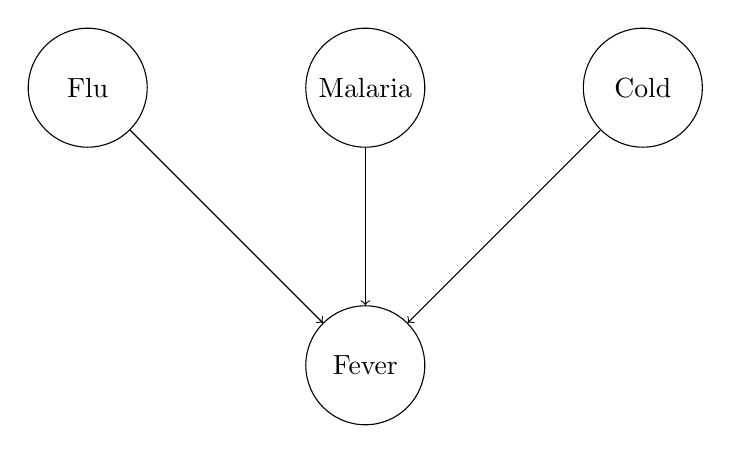
\begin{tikzpicture}[
  node distance=2cm and 2cm,
  mynode/.style={draw,circle,text width=1.2cm,align=center},
]
\node[mynode] (flu) {Flu};
\node[mynode,right=of flu] (malaria) {Malaria};
\node[mynode,right=of malaria] (cold) {Cold};
\node[mynode,below=of malaria] (fever) {Fever};

\path (flu) edge[->] (fever)
(malaria) edge[->] (fever)
(cold) edge[->] (fever)
;
\end{tikzpicture}

The causal relationship between parent and child may be inhibited (e.g. no fever but has flu). Two assumptions:
\begin{itemize}
    \item
        All the possible causes are listed (If some are missing, we can always add a so-called leak node that covers "miscellaneous causes")
    \item
        Inhibition of each parent is independent of any other parent (Whatever inhibits malaria from causing a fever is independet of whatever inhibits flu from causing fever)
\end{itemize}
Given these assumptions, \(Fever\) is false if and only if all its \(true\) parents are inhibited

\(\Rightarrow P(x_i | parents(X_i)) = 1 - \prod_{j:X_j = true} q_j\), where \(q_j\) are the inhibition probabilities.

The full CPT can now be described using \(O(k)\) parameters.

\subsection{Inference in Bayesian Networks (Inference by enumeration)}
The basic task for any probabilistic inference system is to compute the posterior probability distritubtion for a set of \textbf{query variable}(s) \(X\), given some observed \textbf{event} \(e\) - that is, some assignment of values to a set of \textbf{evidence variables} \(E = \{E_1, \dots, E_m\}\). \(Y = \{Y_1, \dots, Y_l\}\) will denote the nonevidence, nonquery variables, also called \textbf{hidden variables}.

\bigbreak

Conditional probabilities can be computed by summing terms from the full joint probability distribution:
\[P(X|e) = \alpha P(X, e) = \alpha \sum_y P(X, e, y)\]
\textit{Reminder:} \(P(X|e) = \frac{P(X,e)}{P(e)} = \alpha P(X,e),\ \alpha = \frac{1}{P(e)}\)

A query can be answered using a Bayesian network by computing sums of products of conditional probabilities from the network.

\textit{Reminder:} \(P(X_1, \dots, X_n) = \prod_{i=1}^n P(X_i | Parents(X_i))\)

\bigbreak

\textbf{Example} (hidden variables: \textit{Earthquake} and \textit{Alarm}):
\begin{align*}
    P(Burglary | JohnCalls = \top, MaryCalls = \top) = P(B | j, m) &= \alpha \sum_e \sum_a P(B, j, m, e, a) \\
    &= \alpha \sum_e \sum_a P(b) P(e) P(a|b,e) P(j|a) P(m|a)\\
    &= \alpha P(b) \sum_e P(e) \sum_a  P(a|b,e) P(j|a) P(m|a)
\end{align*}


\textbf{Variable Elimnation} can make computation increadibly faster in the case of polytrees (there is at most one undirected path between any two nodes in the graph).

General probabilistic inference is \(\#P\)-hard, which is harder then NP. In the hard cases, approxiamation is key.

\subsection{Conclusion}
\begin{itemize}
    \item
        \textbf{Bayesian networks} are a wide-spread tool to model uncertainty, and to reason about it. A BN represents \textbf{conditional independence} relations between random variables. It consists of a graph encoding the variable dependencies, and of conditional probability tables (CPTs).
    \item
        Given a variable order, the BN is small (concerning CPT sizes) if every variable depends only on a few of its predecessors
    \item
        \textbf{Probabilistic inference} requires to compute the probability distribution of a set of query variables, given a set of evidence variables whose values we know. The remaining variables are hidden. 
    \item
        Inference by enumeration takes a BN as input, then applies \textbf{Normalization and Marginalization}, the \textbf{Chain rule}, and exploits conditional independence.
    \item
        \textbf{Variable elimination} avoids unnecessary computation. It runs in polynomial time for polytree BNs. In general, exact probabilistic inference is \(\#P-hard\). Approximate probabilistic inference methods exist.
\end{itemize}

\section{Making Simple Decisions Rationally}
\subsection{Rational Preference}
\textbf{Decision theory} investigates how an agent \(a\) deals with choosing among actions based on the desirability of their outcomes. We restrict ourself to \textbf{episodic} decision theory, which deals with choosing among actions based on the desirabilty of their immediate outcomes. We have to deal with non-deterministic, partially observable environments.

\bigbreak

\(Result(a)\) is a random variable, whose values are possible outcome states of an action. The probability of outcome \(s'\), given evidence observations \(e\), is written
\(P(Result(a) = s' | a,e)\).

The agent's preferences are captured by a \textbf{utility function} \(U(s)\), which assigns a single number to express the desirability of a state. The \textbf{expected utility} of an action given the evidence, \(EU(a|e)\), is just the average utility value of the outcomes, weighted by the probability that the outcome occurs:
\[EU(a|e) = \sum_{s'} P(Result(a) = s'|a,e)U(s')\]

The principle of \textbf{maximum expected utility} (MEU) says that a rational agent should choose the action that maximizes the agent's expected utility:
\[action = argmax_a EU(a|e)\]

\subsubsection{Preference}
An agent chooses among \textbf{outcomes} (\(A, B\), etc.) and \textbf{lotteries}, i.e., situations with uncertain prizes.
\[Lottery \ L = [p_1, S_1; p_2, S_2; \dots p_n, S_n]\]
\begin{itemize}
    \item
        \(A \succ B\): \(A\) \textbf{preffered} over \(B\)
    \item
        \(A \sim B\): \textbf{indifference} between \(A\) and \(B\)
    \item
        \(A \succeq B\): \(A\) prefered over \(B\) or indifferent
\end{itemize}
Six constraint that we require any reasonable preference relation to obey: Orderability, Transitivity, Continuity, Substituability, Monotonicity, Decomposability (Axioms of utility theory).
%\begin{itemize}
 %   \item
 %       Orderability: Given any two lotteries, a rational agent either prefer one to the other or else rate the two as equally preferable.
 %   \item
 %       Transitivity: If an agent prefers \(A\) over \(B\) and \(B\) over \(C\), then the agent must prefer \(A\) over \(C\).
 %   \item
%        Continuity: If some lottery \(B\) is between \(A\) and \(C\) in preference, then there is some probability \(p\) for which the rational agent will be indifferent between getting \(B\) for sure and the lottery that yields \(A\) which \(p\) and \(C\) with \(1-p\).
%    \item
%        Substituability: If an agent is indifferent between two lotteries \(A\) and \(B\), then the agent is indifferent between two more complex lotteries that are the same except that \(B\) is substituted for \(A\) in one of them: \(A \sim B \Rightarrow [p, A; 1-p, C] \sim [p, B; 1-p, C]\). This also holds if we substitute \(\succ\) for \(\sim\) in this axiom.
%    \item
%        Monotonicity: Suppose two lotteries have the same two possible outcomes
%\end{itemize}

\subsubsection{Preference lead to utility}
\begin{itemize}
    \item
        \textbf{Existence of Utility Function:} If an agent's preferences obey the axioms of utility, then there exists a function \(U\) such that \(U(A) > U(B)\) if and only if \(A\) is preferred to \(B\), and \(U(A) = U(B)\) if and only if the agent is indifferent between \(A\) and \(B\).\\
         \[U(A) > U(B) \Leftrightarrow A \succ B\]
    \item
        \textbf{Expected Utility of a Lottery:} The utility of a lottery is the sum of probability of each outcome times the utility of that outcome.
        \[U([p_1, S_1; \dots; p_n, S_n]) = \sum_i p_i U(S_i)\]
\end{itemize}
We call a total preference ordering on states a \textbf{value function} or \textbf{ordinal utility function}.

\textit{Note:} An agent doesn't implicitly have to maximize an utility function. Rational behavior can be generated in any number of ways. By observing a rational agent's preference, however, an observer can construct the utility function that represents what the agent is actually trying to achieve (even if the agent doesn't know it)

\subsubsection{Utility assessment and utility scales}
\underline{Goal:} working out a agent's utility function (\textbf{preference elicitation}). This process involves presenting choices to the agent and using the observed preferences to pin down the underlying utility function.

Fix the utility of a "best possible price" at \(U(S) = u_{\top}\) and a "worst possible catastrophe" at \(U(S) = u_{\bot}\). \textbf{Normalized utilities} use a scale with \(u_{\bot} = 0\) and \(u_{\top} = 1\).

Given a utility scale between \(u_{\bot}\) and \(u_{\top}\), we can assess the utility of any particular prize \(S\) by asking the agent to choose between \(S\) and a \textbf{standard lottery} \([p, u_{\top}; (1-p), u_{\bot}]\). The probability \(p\) is adjusted until the agent is indifferent between \(S\) and the standard lottery. Assuming normalized utilities, the utility of \(S\) is given by \(p\). Once this is done for each prize, the utilities for all lotteries involving those prizes are determined.

\subsection{Multiattribute Utility Functions}
Problems, in which outcomes are characterized by two or more attributes, are handled by \textbf{multiattribute utility theory}. We will call the attributed \(X = X_1, \dots, X_n\); a complete vector of assignments will be \(x = \langle x_1, \dots, x_n \rangle\), where each \(x_i\) is either a numeric or discrete value. We will assume that higher values of an attribute correspond to higher utilities.

\subsubsection{Dominance}
A choice \(S_1\) is said to \textbf{strictly} dominate \(S_2\), iff \(X_i(S_1) > X_i(S_2), \ \forall i\). For the non-deterministic case, all possible concrete outcomes for \(S_1\) have to strictly dominante all possible outcomes for \(S_2\) (very rare).

\begin{center}
    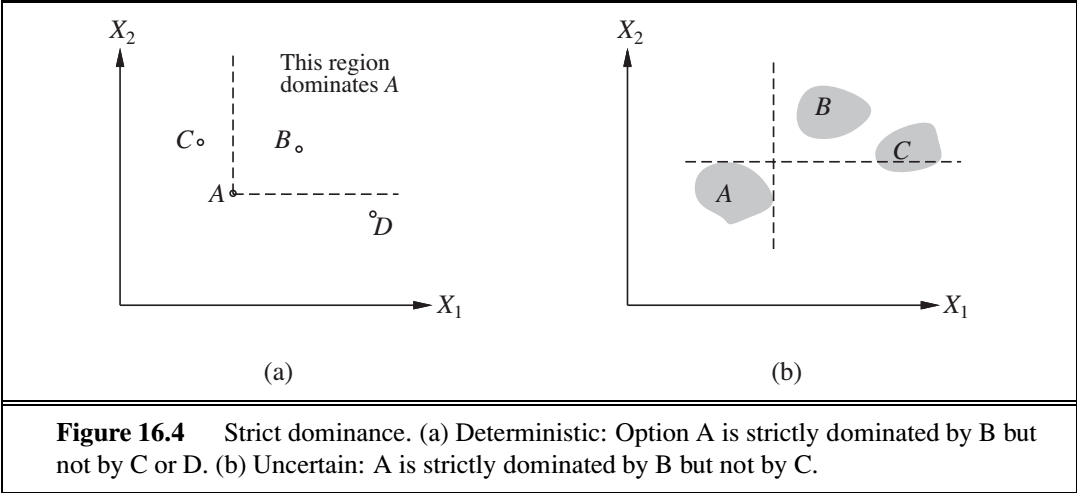
\includegraphics[scale=0.4]{img/stricdom.png}
\end{center}

If two actions \(A_1\) and \(A_2\) lead to probability distributions \(p_1(x)\) and \(p_2(x)\) on attribute \(X\), then \(A_1\) \textbf{statistically dominates} \(A_2\) if
\[\forall x \int_{-\infty}^x p_1(x') dx' \leq \int_{-\infty}^x p_2(x')dx'\]
(the cumulative distribution of \(S_1\) is always to the right of the one for \(S_2\)).

If \(A_1\) stochatically dominates \(A_2\), then for any monotonically nondecreaing utility function \(U(x)\), the expected utility of \(A_1\) is at least as high as the expected utility of \(A_2\). Hence, if an action is stochastically dominated by another action on all attributes, then it can be discarded.

\begin{center}
    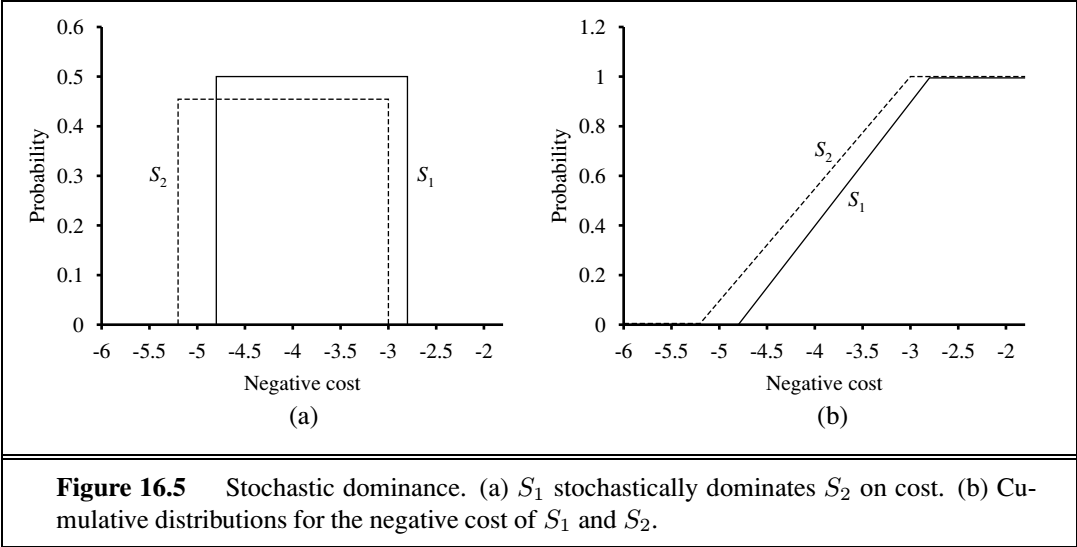
\includegraphics[scale=0.4]{img/statdom.png}
\end{center}

\subsubsection{Preference structure and multiattribute utility}
Suppose we have \(n\) attributes, each of which has \(d\) distinct possible values. To specify the complete utility function \(U(x_1, \dots, x_n)\), we need \(d^n\) values in the worst case. Now, the worst case corresponds to a situation in which the agent's preferences have no regularity at all. Multiattribute utility theory is based on the suppostition that the preferences of typical agents have much more structure than that.

The basic approach is to identify regularities in the preference behavior and to use what are called \textbf{representation theorems} to show that an agent with a certain kind of preference structure has a utility function
\[U(x_1, \dots, x_n) = F[f_1(x_1), \dots, f_n(x_n)]\]
where \(F\) is, we hope, a simple function such as addition.

... whatever (Was wollen sie mir hier genau beibringen Herr Kohlhase?)

\subsection{Decision Networks}
Decision networks combine Bayesian networks with additional node types for actions and utilities.

\subsubsection{Representing a decision problem with a decision network}
In it's most general form, a decision network represents information about the agent's current state, its possible actions, the state that will result from the agent's action, and the utility of that state.

\textbf{Node types:}
\begin{itemize}
    \item
        \textbf{Chance nodes} (oval) represent random variables. Each node has associated with it a conditional distribution that is indexed by the state of the parent nodes.
    \item
        \textbf{Decision nodes} (rectangle) represent points where the decision maker has a choice of actions.
    \item
        \textbf{Utility nodes:} (diamonds) represent the agent's utility function. The utility node has as parents all variables describing the outcome that directly affect utility. Associated with the utility node is a description of the agent's utility as a function of the parents attributes.
\end{itemize}

\begin{center}
    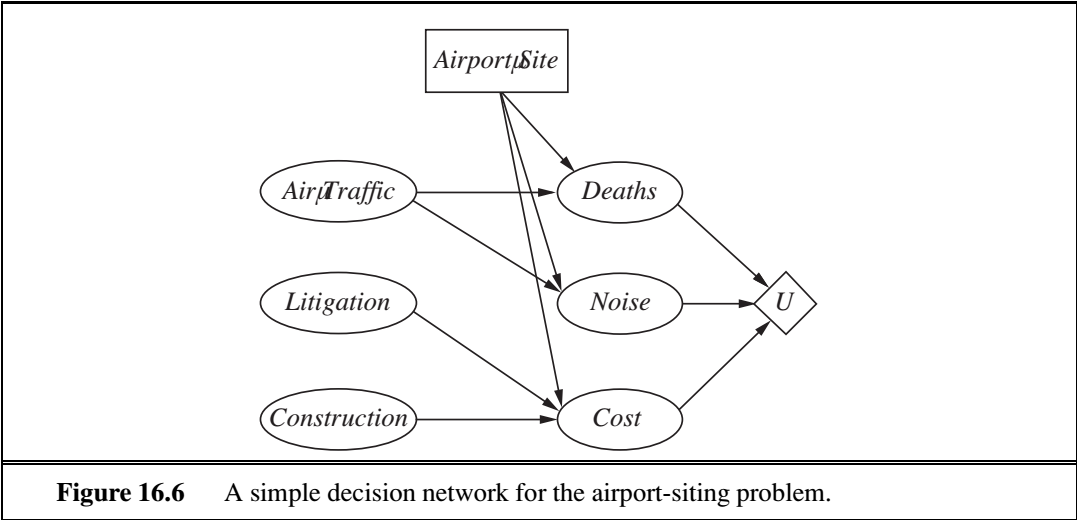
\includegraphics[scale=0.4]{img/airport.png}
\end{center}

Actions are selected by evaluating the decision network for each possible setting of the decision node. 
\textbf{Algorithm:}
\begin{enumerate}
    \item
        Set the evidence variables to the current state
    \item
        For each possible value of the decision node:
        \begin{enumerate}
            \item
                Set the decision node to that value
            \item
                Calculate the posterior probabilities for the parent nodes of the utility node, using a standard probabilistic inference algorithm
            \item
                Calculate the resulting utility for the action
        \end{enumerate}
    \item
        Return the action with the highest utility
\end{enumerate}

\begin{comment}
\subsection{Recap: Agent Architectures based on Belief States}
\begin{center}
    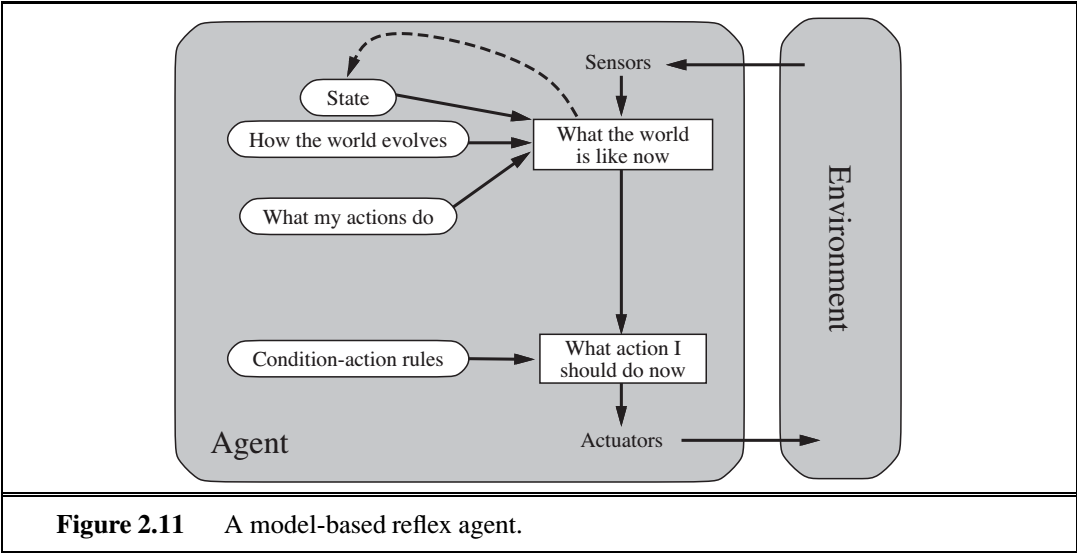
\includegraphics[scale=0.4]{img/refage.png}
\end{center}
The most effective way to handle partial observability is for the agent to keep track of the part of the world it can't see right now.

A stateful reflex agent has a world model consisting of:
\begin{itemize}
    \item
        a \textbf{belief state} that has information about the possible states the world may be in
    \item
        a \textbf{transition model} that updates the belief state based on sensor information and actions
\end{itemize}
The agent environment determines what the world model can be.

\bigbreak

In a fully observable, deterministic environment
\begin{itemize}
    \item
        we can observe the initial state and subsequent states are giben by the actions alone
    \item
        the belief state is a singleton set and the transition model is a function from states and actions to states: a \textbf{transition} function
\end{itemize}

In a fully observable, but stochastic environment
\begin{itemize}
    \item
        the belief state must deal with a set of possible states
    \item
        generalize the transition function to a \textbf{transition relation}
\end{itemize}

In a deterministic, but partially observable environment
\begin{itemize}
    \item
        the belief state must deal with a set of possible states
    \item
        we can use a transition function
    \item
        We need a \textbf{sensor model}, which predicts the influence of percepts on the belief state - during update
\end{itemize}

In a stochastic, partially observable environment
\begin{itemize}
    \item
        mix the ideas from the last two (sensor model + transition relation)
\end{itemize}
\end{comment}



\subsection{The Value of Information}
\textbf{Information value theory} enables an agent to choose what information to acquire.

\subsubsection{Example}
\begin{itemize}
    \item
        Oil company wants to buy one of \(n\) blocks of ocean-drill rights
    \item
        One of the blocks contains oil worth \(C\) dollar, while others are worthless
    \item
        Suppose seismologist offers the company results of a survey of block number 3, which indicates definitively wether the block contains oil
    \item
        How much should the company be willing to pay for the information?
\end{itemize}

With probability \(1/n\), the survey will indicate oil in block 3 and the company will buy block 3 for \(C/n\) dollars

 \(\Rightarrow Profit = C - C/n = (n-1)C/n\)

 With probability \(n-1)/n\), the survey will show that block contains no oil, in which case the company will buy a different block
 
 \(\Rightarrow Expected \ Profit = C/(n-1) - C/n = C/(n-1)n\) 

 Expected profit, given the survey information: \(\frac{1}{n} \times \frac{(n-1)C}{n} + \frac{n-1}{n} \times \frac{C}{n(n-1)} = C/n\)

 Therefore, the company should be willing to pay the seismologist up to \(C/n\) dollars for the information: the information is worth as much as the block itself.

 In general, the value of a given piece of information is defined to be the difference in expected value between best action before and after information is obtained.

\subsubsection{A general formula for perfect imformation}
We assume that exact evidence can be obtained about the value of some random variable \(E_j\) (that is, we learn \(E_j = e_j\), so the phrase \textbf{value of perfect information} (VPI) is used.

Let the agent's initial evidence be \(e\). Then the value of the current best action \(\alpha\) is defined by
\[EU(\alpha|e) = max_{a} \sum_{s'} P(Result(a) = s'|a, e) U(s')\]
and the value of the next best action (after the new evidence \(E_j = e_j\) is obtained) will be 
\[EU(\alpha_{e_j}|e, e_j) = max_a \sum_{s'} P(Result(a) = s' | a, e, e_j) U(s')\]
But \(E_j\) is a random variable whose value is currently unknown, so to determine the value of discovering \(E_j\), given current information \(e\) we must average over all possible values \(e_{jk}\) that we might discover, using our current beliefs about its value:
\[VPI_e(E_j) = (\sum_k P(E_j = ejk | e) EU(\alpha_{e_{jk}} | e, E_j = e_{jk})) - EU(\alpha|e)\]

\begin{center}
    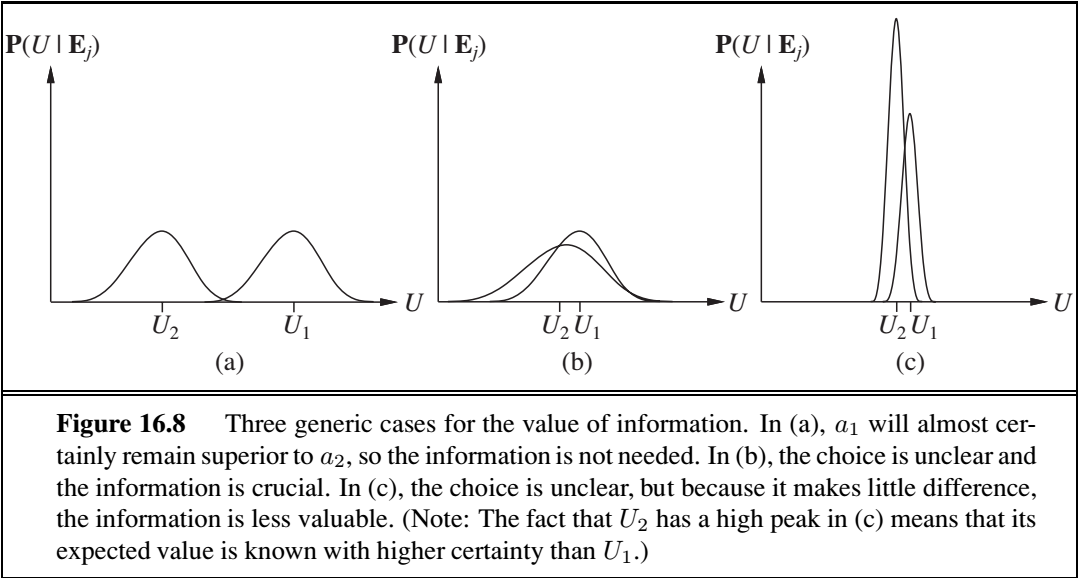
\includegraphics[scale=0.4]{img/vpi.png}
\end{center}

\begin{itemize}
    \item
        Suppose \(a_1\), \(a_2\) represent two different routes through mountain range
    \item
        (a)
        \begin{itemize}
            \item
                \(a_1\) nice and chill, \(a_2\) winding road, might snow as fuck and way might be blocked
            \item
                Clearly: \(U_1 > U_2\)
            \item
                Possibility to obtain satellite images
            \item
                Distribution of new expectations shows that, about 99.9\% of the time the plans won't change
        \end{itemize}
    \item
        (b)
        \begin{itemize}
            \item
                Choosing between two similar roads which could be blocked and we are carrying a seriously injured passenger 
            \item
                \(U_1\) and \(U_2\) are quite close
            \item
                Distributions show that sattelite information might change utilities drastically (because very broad)
        \end{itemize}
    \item
        (c)
        \begin{itemize}
            \item
                Choosing between two dirt roads in summertime, when blockage is unlikely (Utilities pretty close)
            \item
                Distributions show that additional information might quite likely change our plans
            \item
                But: The difference in utility is likely to be very small, so it isn't worth the effort
        \end{itemize}
\end{itemize}

\bigbreak

\textbf{In sum, information has value to the extent that it is likely to cause a change of plan and to the extent that the new plan will be significantly better than the old plan.}

\subsubsection{Implementation of an information-gathering agent}
A sensible agent should ask questions in a reasonable order, should avoid asking questions that are irrelevant, should take into account the importance of each piece of information in relation to its cost, and should stop asking questions when that is appropriate.

We assume that with each observable evidence variable \(E_j\), there is an associated cost, \(Cost(E_j)\). We assume that the result of the action \(Request(E_j)\) is that the next percept provides the value of \(E_j\).

\begin{center}
    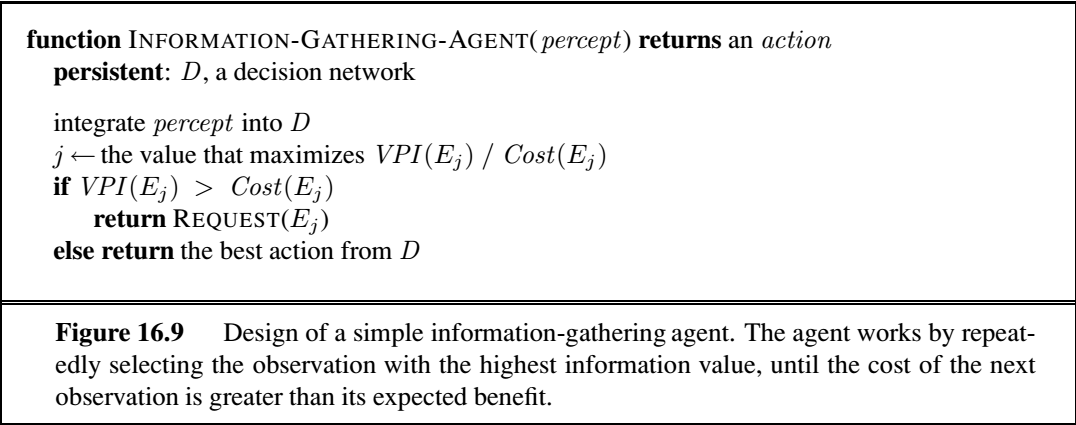
\includegraphics[scale=0.4]{img/vpiag.png}
\end{center}

Form of information gathering: \textbf{myopic}. The algorithm uses the VPI formula shortsightedly, calculating the value of information as if only a single evidence variable will be acquired. If there is no single evidence variable that will help a lot, a myopic agent might hastily take an action when it would have been better to request two or more variables first and then take actions.

\section{Temporal probability models (Probabilistic Reasoning Over Time)}
\subsection{States and observation}
We view the world as a series of snapshots, or \textbf{times slices}, each of which contains a set of random variables, some observable and some not. We will use \(X_t\) to denote the set of state variables at time \(t\), which are assumed to be unobservable, and \(E_t\) to denote the set of observable evidence variables. The observation time \(t\) is \(E_t = e_t\) for some set of values \(e_t\). The state sequence starts at \(t=0\).

\textit{Notation:} \(X_{a:b} = \) set of variables from \(X_a\) to \(X_b\).

\subsection{Transition and sensor models}
Two questions: 
\begin{itemize}
    \item
        How does the world evolve? (\(\rightarrow\) \textbf{transition model})
    \item
        How do evidence variables get their values (\(\rightarrow\) \textbf{sensor model})
\end{itemize}

\bigskip

The \textbf{transition model} specifies the probability distribution over the last state variables given the previous values, that is, \(P(X_t | X_{0:t-1})\).
\begin{itemize}
    \item
        Problem: the set \(X_{0:t-1}\) is unbound in the size as \(t\) increases
    \item
        Solution: \textbf{Markov assumption} - the current state depends only on a \textit{finite fixed number} of previous states  
    \item
        Processes satisfying this assumption are called \textbf{Markov processes} or \textbf{Markov chains} 
    \item
        Another problem: infinetly many possible values of \(t\). Do we need specify a different distribution for each time step?
    \item
        Another solution: We assume that changes in the world state are caused by a \textbf{stationary process}, which doesn't change over time (e.g. \(P(R_t | R_{t-1})\) is the same \(\forall t\))
\end{itemize}

\begin{center}
    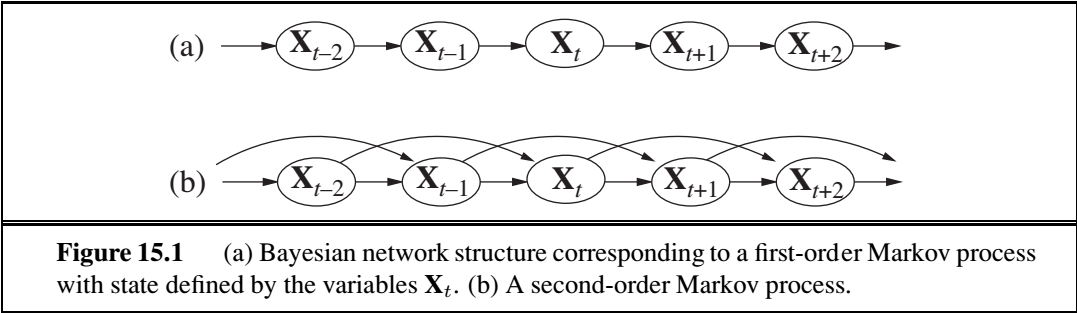
\includegraphics[scale=0.4]{img/markpro.png}
\end{center}

\bigbreak

The \textbf{sensor model} specifies, how evidences are generated (on which state variables they depend). We make the \textbf{sensor Markov assumption}:
\[P(E_t | X_{0:t}, E_{0:t-1}) = P(E_t | X_t)\]

\begin{center}
    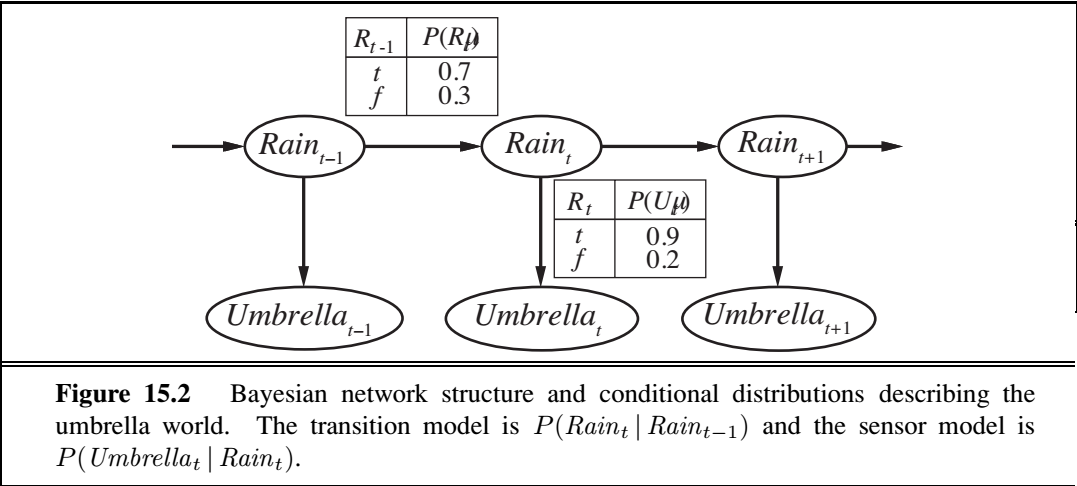
\includegraphics[scale=0.4]{img/transenmod.png}
\end{center}

Additionally, we need to specify an intial state probability \(P(X_0)\).

The complete joint probability distribution over all the variables is (for any \(t\), with first order Markov assumption) given by
\[P(X_{0:t}, E_{1:t}) = P(X_0) \prod_{i=1}^t P(X_i|X_{i-1}) P(E_i | X_i)\]
and consists of initial state probability, the transition model and the sensor model.

One problem with the first order Markov assumption is, that it might not model the real world apropriatly. Possible fixes:
\begin{itemize}
    \item
        Increase order of Markov process
    \item
        Augment state, e.g. \(Season_t\), \(Temp_t\), \(Pressure_t\) 
\end{itemize}

\subsection{Inference in Temporal Models}
\textbf{Inference tasks:}
\begin{itemize}
    \item
        \textbf{Filtering:} computing the \textbf{belief state} - the posterior distribution over the most recent state - given all evidence to date. In our example, we wish to compute \(P(X_t|e_{1:t})\). Filtering is what a rational agent does to keep track of the current state so that rational decisions can be made
    \item
        \textbf{Prediction:} computing the posterior distribution over the future state, given all evidence to date. That is, we wish to compute \(P(X_{t+k}|e_{1:t})\) for some \(k>0\)
    \item
        \textbf{Smoothing:} computing the posterior distribution over a past sate, given all evidence up to the present. That is, we wish to compute \(P(X_k|e_{1:t})\) for some \(k\) such that \(0 \leq k < t\). Smoothing provides a better esimate of the state than was available at the time, because it incorporates more evidence
    \item
        \textbf{Most likely explanation:} Given a sequence of observations, we might wish to find the sequence of states that is most likely to have generated those observations. That is, we wish to compute \(argmax_{x:t} P(x_{1:t}|e_{1:t})\)
\end{itemize}

\subsubsection{Filtering and prediction}
Given the filtering result up to time \(t\), the agents needs to compute the result for \(t+1\) from the new evidence \(e_{t+1}\),
\[P(X_{t+1} | e_{1:t+1}) = f(e_{t+1}, P(X_t|e_{1:t}))\]
for some function \(f\). This process is called \textbf{recursive estimation}.

Two part process: first, the current state distribution is projected forward from \(t to t+1\); then it is updated using the new evidence \(e_{t+1}\).
\begin{align*}
    P(X_{t+1} | e_{1:t+1}) &= P(X_{t+1} | e_{1:t}, e_{t+1})\\
    &= \alpha P(e_{t+1} | X_{t+1}, e_{1:t}) \ P(X_{t+1} | e_{1:t})\\
    &= \alpha P(e_{t+1} | X_{t+1}) \ P(X_{t+1} | e_{1:t})
\end{align*}

\(P(e_{t+1} | X_{t+1})\) is given by the sensor model. We obtain the other term by conditioning on the current state \(X_t\):
\begin{align*}
    P(X_{t+1} | e_{1:t}) &= \sum_{x_t} P(X_{t+1} | x_t, e_{1:t}) P(x_t | e_{1:t})\\
    &= \sum_{x_t} P(X_{t+1} | x_t)P(x_t|e_{1:t})
\end{align*}

so

\[P(X_{t+1} | e_{1:t+1}) = \alpha P(e_{t+1} | X_{t+1}) \ \sum_{x_t} P(X_{t+1} | x_t)P(x_t|e_{1:t})\]




In the summation, the first factor comes from the transition model and the second comes from the current state distribution. Hence, we have the desired recursive formulation. 
We can think of the filtered estimate \(P(X_t | e_{1:t})\) as a message \(f_{1:t}\) that is propagated forward along the sequence, modified by each transition and updated by each new observation. 
The process is given by \(f_{1:t+1} = \alpha FORWARD(f_{1:t}, e_{t+1})\).

\bigbreak

\textbf{Prediction} is simply filtering without new evidence, 
\[P(X_{t+k+1} | e_{1:t}) = \sum_{x_{t+k}} P(X_{t+k+1}|x_{t+k}) P(x_{t+k}|e_{1:t})\]

As \(k\ \rightarrow \infty\) the predicted distribution tends to converge to a fixed point, after which it remains constant for all time. This is the stationay distribution of the Markov process defined by transition model.

\subsubsection{Smoothing}
We can again split the computation into two parts - the evidence up to \(k\) and the evidence from \(k+1\) to \(t\).
\begin{align*}
    P(X_k | e_{1:t}) &= P(X_k | e_{1:k}, e_{k+1:t})\\
    &= \alpha P(X_k | e_{1:k}) P(e_{k+1:t}|X_k, e_1:k)\\
    &= \alpha P(X_j | e_{1:k}) P(e_{k+1:t} | X_k)\\
    &= \alpha f_{1:k} \times b_{k+1:t}
\end{align*}

The backward message \(b_{k+1:t}\) can be computed by a recursive process that runs \textit{backward} from \(t\).

\begin{align*}
    P(e_{k+1:t} | X_k) &= \dots\\
    &= \sum_{x_{k+1}} P(e_{k+1}|x_{k+1}) P(e_{k+2:t}|x_{k+1}) P(x_{k+1}|X_k)
\end{align*}

Using the message notation, we have \(b_{k+1:t} = BACKWARD(b_{k+2:t}, e_{k+1})\).

\begin{center}
    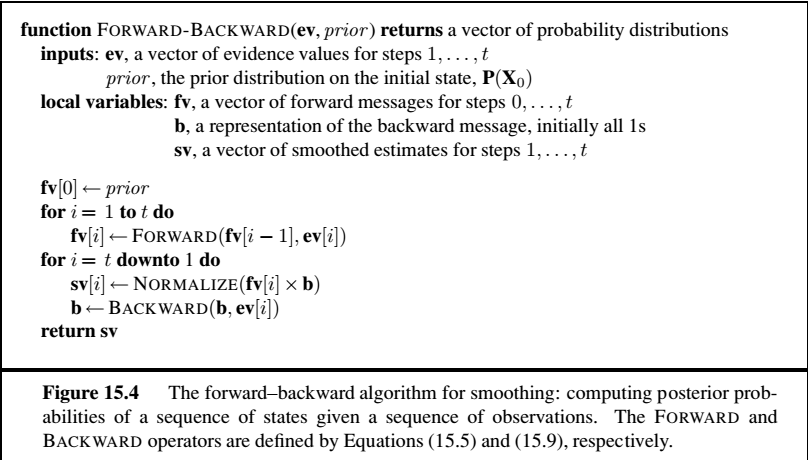
\includegraphics[scale=0.6]{img/fwdbwd.png}
\end{center}

\subsubsection{Finding the most likely sequence}
...

\subsection{HMMs and DBNs}
...

\section{Making Complex decisions}
Here, we deal with \textbf{sequential decision problems}, where the agent's utility depends on a sequence of decisions.

\subsection{Sequential Decision Problems}
\begin{center}
    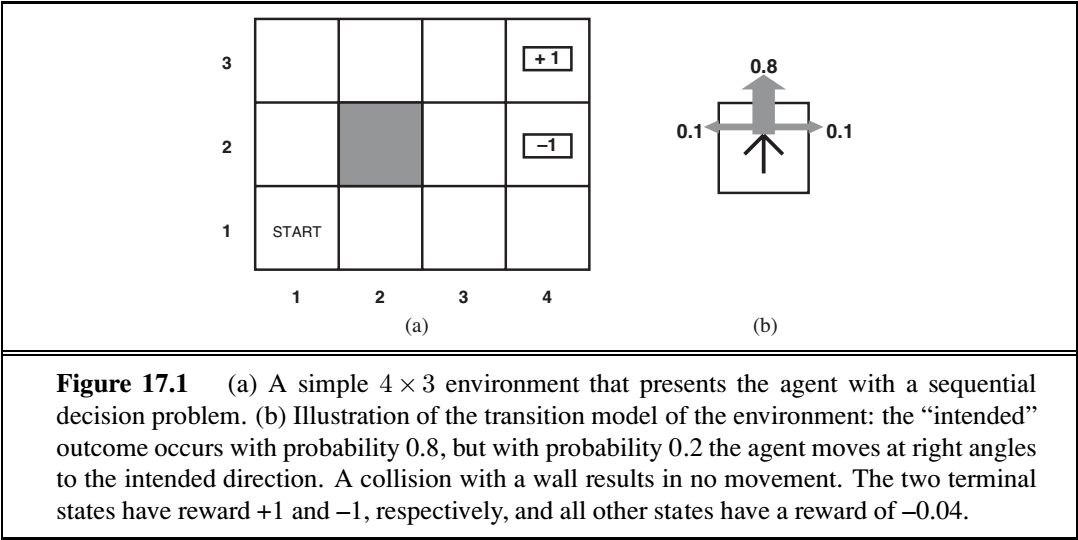
\includegraphics[scale=0.41]{img/4x3.png}
\end{center}
%The \textbf{transition model} desribes the outcome of each action in each state. Here, the outcome is stochastic, so we write \(P(s'|s,a)\) to denote the probability of reaching state \(s'\) if action \(a\) is done in state \(s\). We will assume that the transitions are \textbf{Markovian} in the sense that the probability of reaching \(s'\) from \(s\) depends only on \(s\) and not on the history of earlier states.

%We must specify the utility function for the agent. Because the decision problem is sequential, the utility function will depend on a sequence of states - an \textbf{environment history}. For now, we simply say that the agent receives a reward \(R(s)\) in each state. Also for now the utility of an environment history is the sum of rewards received.

A sequential decision problem for a fully observable, stochastic environment with an Markovian transition model (the probability of reaching \(s'\) from \(s\) depends only on \(s\) and not on the history of earlier states)
 and additive rewards is called a \textbf{Markov decision process}, or \textbf{MDP}, and consists of 
\begin{itemize}
    \item
        a set of states (with an initial state \(s_0\))        
    \item
        a set \(ACTIONS(s)\) in each state
    \item
        a transition model \(P(s'|s,a)\)
    \item
        and a reward function \(R(s)\)
\end{itemize}

\bigbreak

Any fixed action sequence won't solve the problem, because the agent might end up in a state other than the goal. Therefore, a solution must specify what the agnt should do for \textit{any} state that the agent might reach. 

\(\Rightarrow\) Policy \(\pi\), where \(\pi(s)\) is the action recommended by the policy \(\pi\) for state \(s\).

Each time a given policy is executed starting from the initial state, the stochastic nature of the environment may lead to a different enviornment history. The quality of a policy is therefore measured by the expected utility of the possible environment histories generated by the policy. An \textbf{optimal policy} is a policy that yields the highest expected utility and is denoted as \(\pi^*\).

The careful balancing of risk and reward is a characteristic of MDPs that does not arise in deterministic search problems.

\begin{center}
    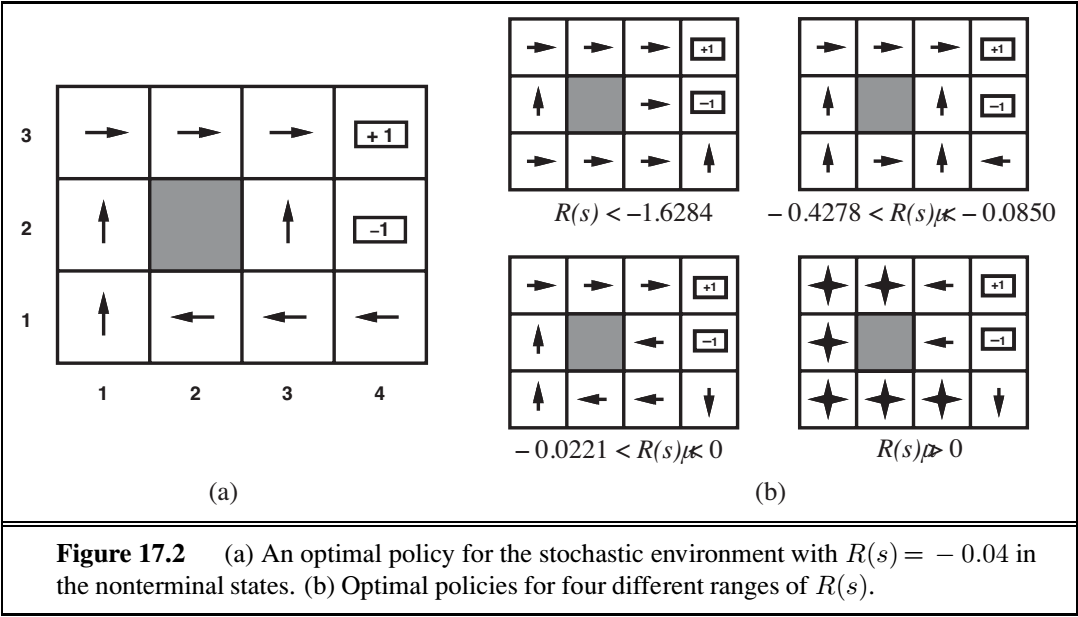
\includegraphics[scale=0.4]{img/4x3cont.png}
\end{center}


\subsubsection{Utilities over time}
Utility function on environmental histories: \(U_h([s_0, s_1, \dots, s_n])\)

\textbf{Finite horizon}: there is a fixed time \(N\) after which nothin matters - the game is over so to speak (\(U_h([s_0, \dots, s_{N+k}]) = U_h([s_0, \dots, s_N])\)). With a finite horizon, the optimal action in a given state could change over time (because for example, the time is running out and I have to take more risk in order to achieve a goal). We say that the optimal policy for a finite horizon is \textbf{nonstationary}.

\textbf{Inifinte horizon}: With no fixed time limit, there is no reason to behave differently in the same state at different times. Hence, the optimal action depends only on the current state, and the optimal policy is \textbf{stationary}.

\bigbreak

We assume that preferences on state sequences are \textbf{stationary},
\[([s, s_0, s_1, s_2 \dots] \succ [s, s_0', s_1', s_2', \dots]) \Leftrightarrow ([s_0, s_1, s_3 \dots] \succ [s_0', s_1', s_2', \dots]) \]
"If you prefere one future to another starting tomorrow, then you should still prefer that future if it were to start today instead."

Under this assumption, there are only two coherent ways to assign utilities to sequences:
\begin{itemize}
    \item
        \textbf{Additive rewards:} The utility of a state sequence is
        \[U_h(s_0, s_1, s_2, \dots) = R(s_0) + R(s_1) + R(s_2) + \dots\]
    \item
        \textbf{Discounted reward:} The utility of a state sequence is 
        \[U_h(s_0, s_1, s_2, \dots) = R(s_0) + \gamma R(s_1) + \gamma^2 R(s_2) + \dots\]
        where the \textbf{discount factor} \(\gamma\) is a number between \(0\) and \(1\). The discount factor decribes the preference of an agent for current rewards over future rewards (\(\gamma = 1\): additive rewards).
\end{itemize}

When we choose an infinite horizon, environmental histories might be infinitely long, and utilities with undiscounted rewards might be infinte. Comparing state sequences with utility \(+\infty\) is difficult. Three solutions:
\begin{enumerate}
    \item
        With discounted rewards, the utility of an infinite sequence is finite. If \(\gamma < 1\) and rewards are bounded by \(\pm R_{max}\), we have
        \[U_h([s_0, s_1, s_2, \dots]) = \sum_{t=0}^{\infty} \gamma^t R(s_t) \leq \sum_{t=0} ^{\infty} \gamma^tR_{max} = R_{max}/(1-\gamma)\]
    \item
        If the environment contains terminal states and if the agent is guaranteed to get to one eventually (has \textbf{proper policy}), we will never need to compare infinite sequences
    \item
        Infinite sequences can be compared in terms of the \textbf{average reward} per time step
\end{enumerate}

\subsubsection{Optimal policies and the utilities of states}
We assume the agent is in some initial state \(s\) and define \(S_t\) to be the state the agent reaches at time \(t\) when executing a particular policy \(\pi\).

The expected utility obtained by executing \(\pi\) starting in \(s\) is given by
\[U^{\pi}(s) = E[\sum_{t=0}^{\infty} \gamma^t R(S_t)]\]
where the expectation is with respect to the probability distribution over state sequences determined by \(s\) and \(\pi\).

\textbf{Optimal policies:} \(\pi_s^* = argmax_{\pi} U^{\pi}(s)\)

When using discounted utilities with infinite horizons, the optimal policy is independent of the starting state.

The utility function \(U(s)\) (\(= U^{\pi^*(s)}\)) allows the agent to choose the action that maximizes the expected utility of the subsequent state:
\[\pi^*(s) = argmax_{a \in A(s)} \sum_{s'} P(s'|s,a) U(s')\]

\subsection{Value Iteration}
The basic idea is to calculate the utility of each state and then use the state utilities to select an optimal action in each state.

\subsubsection{The Bellman equation for utilities}
The utility of a state is the immediate reward for that state plus the expected discounted utility for the next state, assuming that the agent chooses the optimal action. That is, the utility of a state is given by
\[U(s) = R(s) + \gamma \max_{a\in A(s)} \sum_{s'} P(s'|s,a) U(s')\]
called \textbf{Bellman equation}.

\subsubsection{The value iteration algorithm}
\begin{center}
    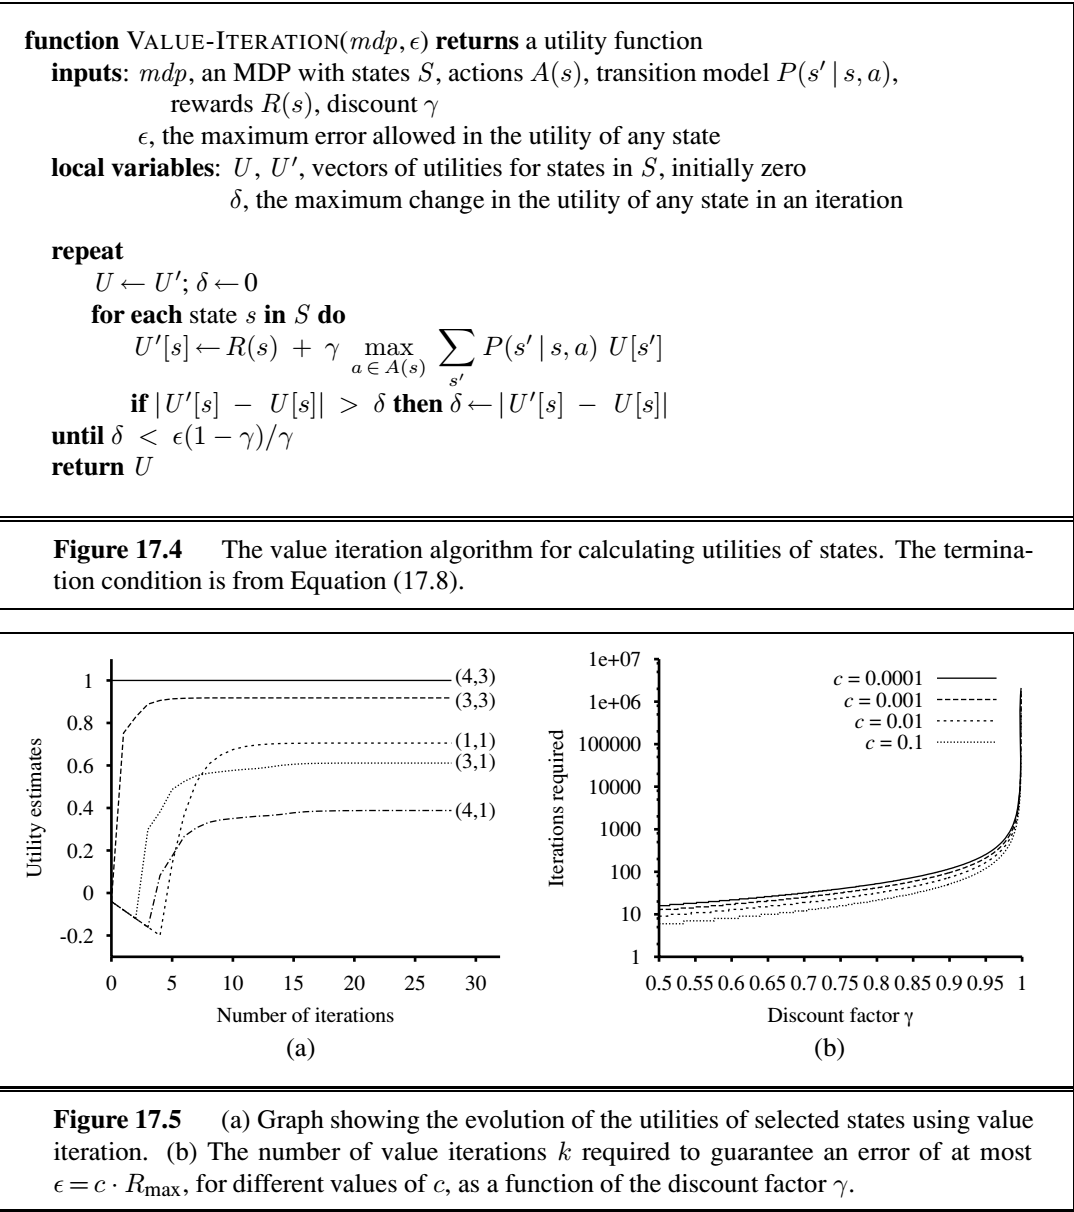
\includegraphics[scale=0.4]{img/valiter.png}
\end{center}

For \(n\) possible states, there are \(n\) Bellman equations, one for each state. The \(n\) (non-linear) equations contain \(n\) unknowns. If we apply the Bellman update infinetly often, we are guaranteed to reach an equilibrium, in which case the final utility values must be solutions to the Bellman equations. In fact, they are also the \textit{unique} solutions, and the corresponding policy is optimal.

\subsection{Policy Iteration}
The policy iteration algorithm alternates the following two steps, beginning from some initilial policy \(\pi_0\):
\begin{enumerate}
    \item
        \textbf{Policy evaluation}: given a policy \(\pi_i\), calculate \(U_i = U^{\pi_i}\), the utility for each state if \(\pi_i\) were to be executed
        \[U_i(s) = R(s) + \gamma \sum_{s'} P(s'|s, \pi_i(s))U_i(s')\]
    \item
        \textbf{Policy improvement}: calculate a new MEU policy \(\pi_{i+1}\), using one-step look-ahead based on \(U_i\)
        \[\pi(s) = argmax_{a \in A(s)} \sum_{s'} P(s'|s,a) U(s')\]
\end{enumerate}
The algorithm terminates when the policy improvement yields no change in the maximum expected utilities. The important point is that these equations are linear, because the max operator has been removed. For \(n\) states, we have \(n\) linear equations with \(n\) unknowns, which can be solved exactly in time \(O(n^3)\).

\subsection{Partially Observable MDPs}
In an \textbf{partially observable} environment, the agent does not necessarily know which state it is in, so it cannot execute the action \(\pi(s)\) recommended for that state. Furthermore, the utility of a state \(s\) and the optimal action in \(s\) depend not just on \(s\), but also on how much the agent knows when it is in \(s\). We cannot avoid POMDPs, because the real world is one.

\subsubsection{Definition of POMDPs}
A partially observable MDP is a MDP (transition model, actions, reward function) together with an \textbf{observation model} \(O\) that is stationary and has the sensor Markov property: \(O(s,e) = P(e|s)\).

The optimal policy in an POMDP is a function \(\pi(b)\) where \(b\) is the \textbf{belief state} (probability distribution over states). The optimal action depends only on the agent's current belief state, it does not depend on the actual state.

If \(b(s)\) (the probability/belief degree that agent is in \(s\)) is the previous belief state and the agent does an action \(a\) and then perceives \(e\), then the new belief state is
\[b'(s') = \alpha P(e|s') \sum_s P(s'|s,a)b(s)\]

\textbf{POMDP decision cycle}:
\begin{itemize}
    \item
        Given the current belief state \(b\), execute the action \(a=\pi^*(b)\)
    \item
        Receive percept \(e\)
    \item
        Update the current belief state and repeat
\end{itemize}

\bigbreak

... Sehr viel exotischer Stuff. Think I'll skip this, sorry Mr. Prof. No hate.

\section{Learning from Examples}
An agent is \textbf{learning} if its improving its performance on future tasks after making observations about the world.

Reasons for Learning:
\begin{itemize}
    \item
        The designer might not anticipate all possible situations that the agent might find itself in
    \item
        The designer can not anticipate all changes over time
    \item
        Sometimes human programmers have no idea how to program a solution themselves
\end{itemize}

\subsection{Forms of Learning}
Any component of an agent can be improved by learning from data. Improvements, and the techniques used to make them, depend on four major factors:
\begin{itemize}
    \item
        Which component is to be improved
    \item
        What prior knowledge the agent already has
    \item
        What representation is used for the data and the component
    \item
        What feedback is available to learn from ((semi-)supervised, unsupervised or reinforcement)
\end{itemize}

\subsection{Supervised Learning}
Given a \textbf{training set} of \(N\) example input-output pairs
\[(x_1, y_1), (x_2, y_2), \dots, (x_N, y_N)\]
where each \(y_j\) was generated by an unknown function \(y = f(x)\) discover a function \(h\) that approximates the true function \(f\), called \textit{hypothesis}. Learning is a search through the space of possible hypotheses for one that will perfom well, even on new examples beyond the training set. In this case we say the hypotesis \textbf{generalizes} well. Sometimes the function \(f\) is stochastic, why we have to learn a conditional probability \(P(Y|x)\). In general, there is trade-off between complex hypotheses that fit the training data well and simpler hypotheses that may generalize better.

\subsection{Learning Decision Trees}
\subsubsection{The decision tree representaion}
For the moment we restrict ourselfs to a Boolean classification.

A decision tree reaches its decision by performing a sequence of tests. Each internal node corresponds to a test of the value of one of the input attributes, \(A_i\), and the branches from the node are labled with the possible values of the attributes, \(A_i = v_{ik}\).

\subsubsection{Inducing decision trees from examples}
Examples: pairs of \((x,y)\), where \(x\) is a set of values for the input attributes and \(y\) is a single Boolean output value.

It is an intractable problem to find the smallest consistent tree. With some simple heuristic however, we can find a good approximate solution: a small, but not smallest consistent tree.

The Decision-Tree-Learning algorithm adopts a greedy divide-and-conquer strategy: always test the most important attribute first (which makes the most difference to the classification of an example). This test divides the problem up into smaller subproblems that can then be solved recursively.

\bigbreak

\textit{Four cases for recursion:}
\begin{enumerate}
    \item
        If the remaining examples are all positive or negative, we are done.
    \item
        If there are some positive and some negative examples, then choose the best attribute to split them
    \item
        If there are no examples left, it means that no example has been observed for this combination of attribute values, and we return plurality classification of all the examples that were used in constructing the node's parant
    \item
        If there are no attributes left, but both positive and negative examples, it means that these examples have exactly the same description, but different classifications \(\rightarrow\) error or noise in data. Return plurality
\end{enumerate}

\begin{center}
    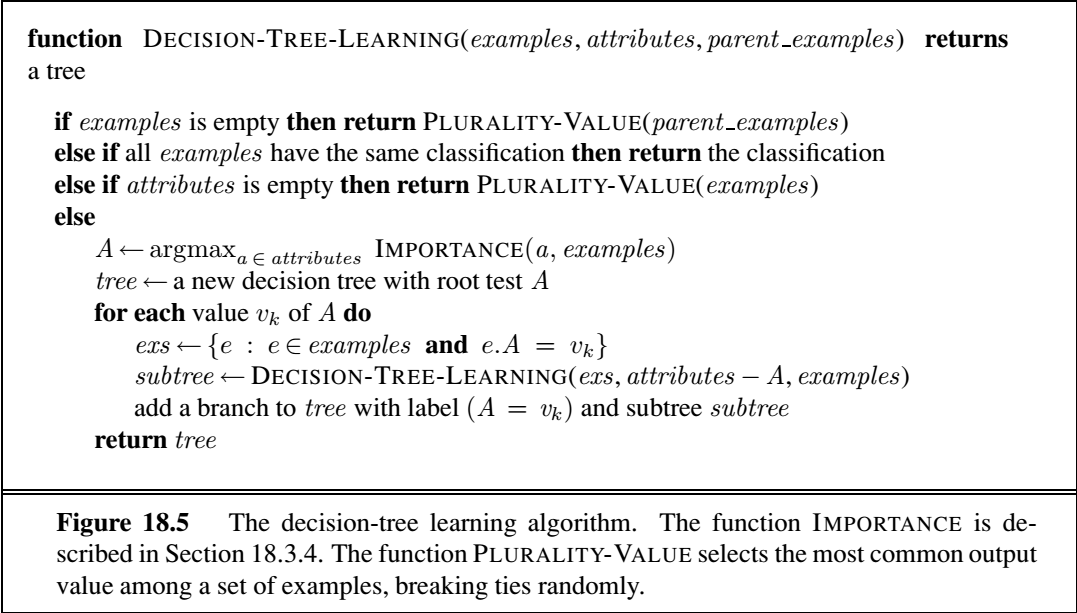
\includegraphics[scale=0.4]{img/dectree.png}
\end{center}

\subsubsection{Choosing attribute tests}
A perfect attribute divides the examples into sets, each of which are all positive or all negative and thus will be leaves of the tree. We will use the notion of information gain, which is defined in terms of \textbf{entropy}.

Entropy is a measure of the uncertainty of a random variable; acquisition of information corresponds to reduction in entropy. In general, the entropy of a random variable \(V\) with values \(v_k\), each with probability \(P(v_k)\), is defined as
\[H(V) = \sum_k P(v_k) log_2 \frac{1}{P(v_k)} = - \sum_k P(v_k) log_2 P(v_k).\]
Entropy for boolean variable, which is true with probability \(q\):
\[B(q) = -(q \ log_2(q) + (1-q) log_2 (1-q))\]
If a training set contains \(p\) positive and \(n\) negative examples, then the entropy of the goal attribute on the whole set is
\[H(Goal) = B(\frac{p}{p+n})\]

An attribute \(A\) with \(d\) distinct values divides the training set \(E\) into \(E_1, \dots, E_d\). Each subset has \(p_k\) positive examples, so if we go along that branch, we will need an additional \(B(p_k/(p_k+n_k))\) bits of information to answer the question. A randomly chosen example from the training set has the \(k\)th value for the attribute with probability \((p_k + n_k)/(p + n)\), so the expected entropy remaining after testing value \(A\) is
\[Remainder(A) = \sum_{k=1}^d \frac{p_k + n_k}{p+n} B (\frac{p_k}{p_k + n_k})\]
The \textbf{information gain} from the attribute test on \(A\) is the expected reduction in entropy:
\[Gain(A) = B(\frac{p}{p+n}) - Remainder(A)\]

\subsubsection{Generalization and overfitting}
Possible problem: \textbf{overfitting}

Solution: \textbf{decision tree pruning}
        
Look at test node that has only leaf nodes as descendant. If the test appears to be irrelevant-detecting only noise in the data-then we eliminiate the test, replacing it with a leaf node (\(\rightarrow\) good indicator: information gain).

...

\subsection{Evaluating and Choosing the Best Hypothesis}
We want to learn a hypothesis that fits the \textbf{future data best}.

\textbf{Future data:}
We make the \textbf{stationary} assumption over future data: that there is a probability distribution over examples that remain stationary over time. Each examples data point is a random variable \(E_j\) whose observed value \((e_j = (x_j, y_j)\) is sample from that distribution, and is independent of the previous examples:
\[P(E_j | E_{j-1}, \dots) = P(E_j)\] 
and each example has an identical prior probability distribution:
\[P(E_j) = P(E_{j-1}) = \dots\]
(Identisch verteilte Zufallsvariablen bestizen alle dieselbe Verteilung, nehmen also mit gleicher Wahrscheinlichkeit gleiche Werte an, beinflussen sich aber nicht gegenseitig)

\bigbreak

\textbf{Best:} We define the \textbf{error rate} of a hypothesis as the proportion of mistakes it makes - the proportion of times \(h(x) \neq y\) for an example \((x,y)\).

\textbf{holdout cross-validation}: Take one portion of the data for training, and the other portion for testing.

\textbf{k-fold-cross-validation}: We perfom \(k\) rounds of learning, where \(\frac{1}{k}\) portion is used for testing.

\textbf{leave-one-out-cross-validation}: \(k=\) number of data samples

It is necessary to further take a part of your test set as a \textbf{validation set} to tune the parameters of your model, because doing so with your test set may make the hypothsis not genalize well.

\subsubsection{Model selection: Complexity versus goodness of fit}
Finding the best hypothesis are two tasks: \textbf{model selection} (define hypothsis space) and \textbf{optimization} (find best hypothesis within that space). Use the validation set for optimization.

\subsubsection{From error rates to loss}
\begin{itemize}
    \item
        Absolute value loss:  \(L_1(y, \hat{y}) = \abs{y - \hat{y}}\) 
    \item
        Squared error loss:  \(L_1(y, \hat{y}) = (y - \hat{y})^2\) 
    \item
        0/1 loss: \(L_{0/1}(y, \hat{y}) = 0  \ or \ 1\)
\end{itemize}

Generalization Loss:
\[GenLoss_L(h) = \sum_{(x,y) \in \eta} L(y, h(x)) P(x,y)\]

Beause \(P(x,y)\) is not known, the learning agent can only estimate generalization loss with \textbf{empirical loss}:
\[EmpLoss_{L,E} (h) = \frac{1}{N} \sum_{(x,y) \in E} L(y, h(x))\]

\subsection{The Theory of Learning}
\textbf{Computational learning theory}: Any hypothesis that is seriously wrong will almost certainly be found out with high probability after a small number of examples, because it will make an incorrect prediction. Thus, any hypothesis that is consistent wit ha sufficiently large set of training examples is unlikely to be seriouly wrong: that is, it must be \textbf{probably approximately corret}.

Any learning algorithm that return hypotheses that are probably approximately corret is called a \textbf{PAC learning} algorithm.

Axioms for PAC learning:
\begin{itemize}
    \item
        Stationarity: \(P(E) = P(X, Y)\) 
    \item
        True function \(f\) is deterministic and a member of the hypothesis class \(\mathcal{H}\) that is being considered
\end{itemize}

\bigbreak

\textbf{Error rate} of a hyposthesis \(h\) is defined as
\[error(h) = GenLoss_{L_{0/1}}(h) = \sum_{x,y} L_{0/1}(y, h(x)) P(x,y)\]
In other words, \(error(h)\) is the probability that \(h\) missclassifies a new example.

A hypothesis \(h\) is \textbf{approximately correct} if \(error(h) \leq \epsilon\), where \(\epsilon\) is a small constant. The hypothesis space containing all the bad ones is called \(\mathcal{H}_{bad}\).

\bigbreak

The probability, that a "seriously wrong" hypothesis \(h_b\) (with \(error(h_b) > \epsilon\)) is consistent with the first \(N\) examples is
\[P(h_b \text{ agrees with \(N\) examples}) \leq (1-\epsilon)^N\]
and
\[P(\mathcal{H}_{bad} \text{ constains a consisten hypothesis)} \leq \abs{\mathcal{H}_{bad}} (1-\epsilon)^N \leq \abs{\mathcal{H}} (1-\epsilon)^N\]

\textit{How many samples do we need, in order to be safe?}

We would like to reduce the probability of this event below some small numer \(\delta\):
\[\abs{\mathcal{H}} (1-\epsilon)^N \leq \delta.\]
It follows that
\[N \geq \frac{1}{\epsilon} (ln\frac{1}{\delta} + ln \abs{\mathcal{H}})\]
Thus, if a learning algorithm return a hypothesis that is consistent with this many examples, then with probability at least \(1-\delta\) it has error at most \(\epsilon\). \(N\) is called the \textbf{sample complexity} of the hypothesis space.

\subsection{Regression and Classification with Linear Models}
\subsubsection{Univatiate linear regression}
Goal: find \(h_w(x) = w_1 x + w_0\) that best fits the data

Squared loss function: \(Loss(h_w) = \sum_{j=1}^N L_2(y_j, h_w(x_j)) = \sum_{j=1}^N (y_j - (w_1x_j + w_0)\)

We would like to find \(w^* = argmin_w Loss(h_w)\), which has a closed form solution.

\bigbreak

If there is no closed form solution, we usually do a \textbf{gradient descent}:
\begin{enumerate}
    \item
        \(w \leftarrow\) any point in the parameters space
    \item
        for each \(w_i\) in \(w\) do: \(w_i \leftarrow w_i - \alpha \frac{\partial}{\partial w_i} Loss(w)\)
    \item
        Repeat 2 until convergence
\end{enumerate}

\subsubsection{Multivariate linear regression}
...

\subsubsection{Linear classifiers with a hard threshold}
A decision boundary is a line (or surface) that separates two classes. 

The decision function is given by \(h_w(x) = 1 \ if \ w\cdot x \geq\) 0 and 0 otherwise.

Perceptron learning rule: \(w_i \leftarrow \alpha \cdot (y - h_w(x)) \cdot x_i\)

\subsubsection{Linear Classification with logistic regression}
Idea: softening the threshold function - approximating the hard threshold with a continous, differentiable function.

\[Logistic(z) = \frac{1}{1+e^{-z}}\]
and
\[h_w(x) = Logisitic(w \cdot x) = \frac{1}{1+e^{-w\cdot x}}\]

The process of fitting the weights of this model to minimize loss on a data set is called \textbf{logistic regression}. 

\subsection{Artificial Neural Networks}
\begin{center}
    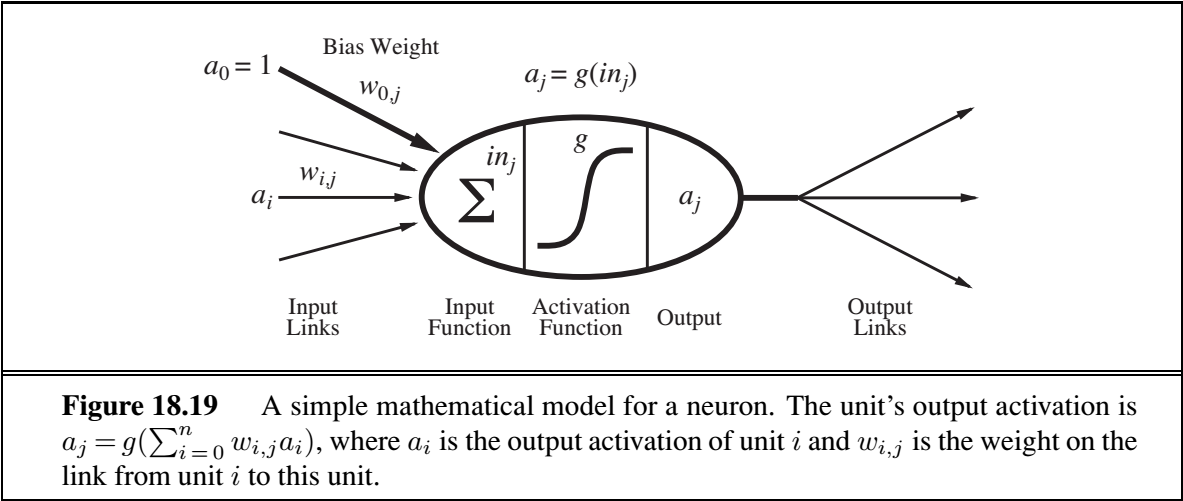
\includegraphics[scale=0.4]{img/neuron.png}
\end{center}

\subsubsection{Neural network structures}
\begin{itemize}
    \item
        Neural networks are composed of nodes or \textbf{units} connected by directed \textbf{links}.
    \item
        A link from unit \(i\) to \(j\) serves to propagate the \textbf{activation} \(a_i\) from \(i\) to \(j\)
    \item
        Each link has a numeric weigth \(w_{i,j}\) associated with it
    \item
        Each unit has a dummy input \(a_0\) with an associated weight \(w_{0,j}\) (\textbf{bias term})
    \item
        Each unit \(j\) computes a weighted sum of its inputs:
        \[in_j = \sum_{i=1}^n w_{i,j} a_i\]
    \item
        Then it applies an \textbf{activation function} \(g\) to this sum to derive
        \[a_j = g(in_j) = g(\sum_{i=1}^n w_{i,j} a_i)\]
    \item
        feed-forward network form a directed acyclic graph, recurrent network feeds its outputs back into its own inputs
\end{itemize}

\subsubsection{Single-layer feed-forward neural networks}
\begin{itemize}
    \item
        A perceptron with \(m\) outputs is really \(m\) seperate networks, because each weight affects only one of the outputs
    \item
        Single perceptron can not learn XOR, because not linearily seperable
\end{itemize}

\subsubsection{Multilayer feed-forward neural networks}
\textit{Question: How do we train such networks?}

Think of the network as a function \(h_w(x)\) parameterized by the weights \(w\). As long as we can calculate the derivatives of this function with respect to the weights, we can use the gradient-descent loss-minimization method to train a network.

It is possible to represent any continous function of the inputs with arbitraty accuracy.

\subsubsection{Learning in multilayer networks}
For the \(L_2\) loss, we have, for any weight \(w\) (because it is additive across the components of the error vector \(y - h_w(x)\):
\[\frac{\partial}{\partial w} Loss(w) = \frac{\partial}{\partial w} \abs{y-h_w(x)}^2 = \frac{\partial}{\partial w} \sum_k (y_k - a_k)^2 = \sum_k \frac{\partial}{\partial w} (y_k - a_k)^2\]

The major complication comes from the addition of hidden layers to the networks. Whereas the error \(y -h_w\) at the output layer is clear, the error at the hidden layers seems mysterious because the training data do not say whay value the hidden nodes should have \(\rightarrow\) \textbf{back-propagate} the error from the output layer to the hidden layers.

Update rule at output layer:
\[w_{j,k} \leftarrow w_{j,k} + \alpha \times a_j \times \Delta_k\]
\[\Delta_k = Err_k \times g'(in_k), \ Err_k = (y-h_w)_k\]

The idea is that hidden node \(j\) is "responsible" for some fraction of the error \(\Delta_k\) in each of the output nodes to which it connects. Thus, the \(\Delta_k\) values are divided according to the strength of the connection between the hidden node and the output node and a backpropagated to provide the \(delta_j\) values for the hidden layer:
\[w_{i,j} \leftarrow w_{i,j} + \alpha \times a_i \times \Delta_j\]
\[\Delta_j = g'(in_j) \sum_k w_{j,k} \Delta_k\]

The backpropagation process can be summarized as follows:
\begin{itemize}
    \item
        Compute the \(\Delta\) values for the output units, using the observed error
    \item
        Starting with outer layer, repeat the following for each layer in the network, until the earliest hidden layer is reached:
        \begin{itemize}
            \item
                Propagate the \(\Delta\) values back to the previous layer
            \item
                Update the weights between the two layers
        \end{itemize}
\end{itemize}

\subsection{Support Vector Machines}
Properties:
\begin{enumerate}
    \item
        SVMs construct a \textbf{maximum margin seperator} - a decision boundary with the largest possible distance to example point
    \item
        SVMs can embed the data into a higher-dimensional space, using the so-called kernel-trick. The high-dimensional linear seperator is actually nonlinear in the original space
\end{enumerate}

The seperator is deined as the set of points \(\{x: w\cdot x + b = 0\}\). Solution can be found by solving
\[argmax_{\alpha} \sum_j \alpha_j - \frac{1}{2} \sum_{j,k} \alpha_j \alpha_k y_j y_k (x_j \cdot x_k)\]
subject to the constraints \(\alpha_j \geq 0\) and \(\sum_j \alpha_j y_j = 0\). 

Our \(w\) then is \(w = \sum_j \alpha_j x_j\) and
\(h(x) = sign(\sum_j \alpha_j y_j (x \cdot x_j) - b)\).

\bigbreak

We see that the data enter the expression only in the form of dot products of pairs of points. We can use the \textbf{kernel trick}: A dot product in a higher dimensional space can be evaluated via a kernel function, without explicitly transforming the data into a higher dimensional space.

\textbf{Mercers theorem} tells us that any "reasonable" kernel function (matrix \(K_{jk} = K(x_j ,x_k)\) is positive definite) corresponds to some feature space.

\section{Knowledge in Learning}
\textbf{In which we examine the problem of learning when you know something already}

\subsection{A Logical Formulation of Learning}
Look at examples described by attribues, e.g. \(Alternate, Bar, Fri/Set\)...

Let us generically call the \(i\)th exmample \(X_i\). We will use the notation \(D_i(X_i)\) to refer to the descprition of \(X_i\), where \(D_i\) can be any logical expression, e.g. \(Alternatve(X_i) \land \lnot Bar(X_i) \dots\). The classification of the example is given by a literal using the goal predicate, e.g. \(WillWait(X_i)\).

The aim of inductive learning in general is to find a hypothesis that classifies the examples well to new exmaples:
\[\forall Goal(x) \Leftrightarrow C_j(x)\]
where \(C_j(x)\) is a candidate definition - some expression involving the attribute predicates.

\begin{center}
    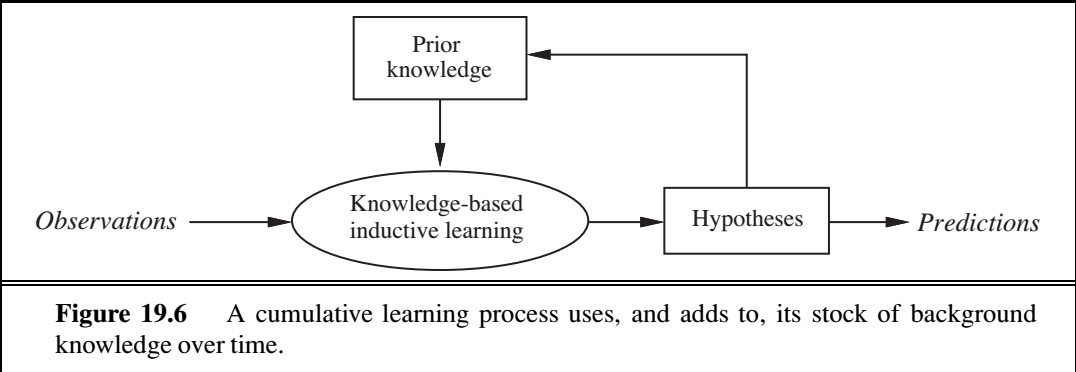
\includegraphics[scale=0.4]{img/cumlearn.png}
\end{center}

\subsection{Explanation-Based Learning}
Is a method for extraction general rules from individual observations.

\textit{Example:} We would like to be able to extract the general rule that for any arithmetic unknown \(u\), the derivative of \(u^2\) w.r.t \(u\) is \(2u\):
\[ArithmeticUnknown(u) \Rightarrow Derivative(u^2, u) = 2u\]  
\subsubsection{Extracting general rules from examples}
The basic idea is first to construct an explanation of the observation unsing prior knowledge, and then establish a definition of the class of cases for which the same explanation structure can be used.

\textbf{... Ich check garnix, scheiss auf Logik!}

\section{Learning Probabilistic Models}
\subsection{Statistical Learning}
\textbf{Bayesian learning} simply calculates the probability of each hypothesis, given the data, and makes predictions on that basis. Let \(D\) represent the data, with observed value \(d\); then the probability of each hypothesis is obtained by Bayes' rule:
\[P(h_i | d) = \alpha P(d|h_i) P(h_i)\]
where the observations are assumed to be independent and identically distributed (i.i.d), and so
\[P(d | h_i) = \prod_j P(d_j|h_i)\]
where \(p(h_i)\) is called the \textbf{hypothesis prior} and \(P(d|h_i)\) the \textbf{likelihood} of the data under each hypothesis.

Now, suppose we want to make a prediction about an unknown quantity \(X\). Then we have
\[P(X|d) =\sum_iP(X, h_i | d) = \sum_i(P(X | h_i, d) \cdot P(h_i | d) = \sum_i P(X|h_i) P(h_i|d)\]
where we assume that each hypothesis determies a probability over \(X\).

Because of computational cost it is often infeasible to compute all the posterior probabilities for each hypotesis. A very common approximation is to make predictions based on a single \textit{most probable} hypothesis - that is, an \(h_i\) that maximizes \(P(h_i|d)\). This is often called a \textbf{maximum a posteriori} or MAP hypothesis with the assumption \(P(X|d) \approx P(X|h_{MAP})\).

\[h_{MAP} = \argmax_{h} P(h|d) = \argmax_{h} \frac{p(d|h) p(h)}{p(d)} = \argmax_{h} p(d|h) p(h)\]

Another simplification is provided by assuming \textbf{uniform} prior over the space of hypotheses. In that case, MAP learning reduces to choosing an \(h_i\) that maximized \(P(d|h_i)\). This is called a \textbf{maximum-likelihood} (ML) hypothsis with
\[h_{ML} = argmax_h p(h|d)\]

\subsection{Learning with Complete Data}
The general task of learning a probability model, given data that are assumed to be generated from that model, is called \textbf{density estimation}. Here: \textbf{complete} data.

\subsubsection{Maximum-likelihood parameters learning: Discrete models}
We are given a dataset \(d\) of \(N\) candies. Under the hypothesis \(h_{\theta}\), the likelihood of this particular data set is
\[P(d|h_{\theta}) = \prod_{j=1}^N P(d_j| h_{\theta})\]

The maximum-likelihood hypothesis is given by the value of \(\theta\) that maximized this expression The same value is obtained by maximizing the \textbf{log-likelihood},
\[L(d|h_{\theta}) = log P(d | h_{\theta}) = \sum_{j=1}^N log P(d_j | h_{\theta})\]
We differentiate \(L\) with respect to \(\theta\) and set the resulting expression to zero (\(\frac{\partial L(d|h_{\theta})}{\partial \theta} = 0\))

\subsubsection{Naive Bayes models}
The different features (attributes) \(x_1, \dots, x_n\) of an observation are assumed to be statistically independent:
\[P(C_k, x_1, x_2, \dots, x_n) = p(C_k) \prod_{i=1}^n p(x_i | C_k) \]
and
\[P(C_k | x_1, x_2, \dots, x_n) = \frac{p(C_k) \prod_{i=1}^n p(x_i | C_k)}{P(x_1, \dots, x_n} = \alpha \ p(C_k) \prod_{i=1}^n p(x_i | C_k) \]

A deterministic prediction can be obtained by choosing the most likely class.

\end{document}

